\scanpage{9}
\mspage{6}
\[
L^{n-i}|M^i:\quad M^i\longrightarrow M^{2n-i}\quad\text{is an isomorphism.}
\tag*{$(6.1)_i$}
\]
This already implies $(4.1)_i$ and $(4.2)_i$ hence $(3.1)_i$ and $(3.2)_i$; \inserted{\figure{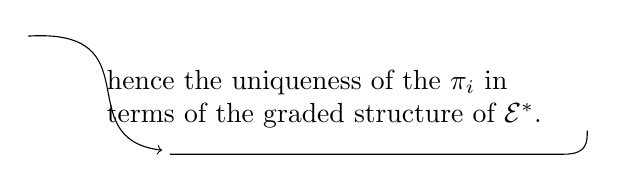
\begin{tikzpicture}[x=1cm,y=1cm]
\node[align=left,text width=6cm] at (1,0) {hence the \uline{uniqueness} of the $\pi_i$ in terms of the graded structure of $\mathcal E^*$.};
\draw[->] (-3,.8) .. controls (-1.4,.9) and (-2.5,-.5) .. (-1.3,-.65);
\draw (-1.2,-.7) -- (3.8,-.7) .. controls (4.1,-.7) and (4.1,-.55) .. (4.1,-.4);
\end{tikzpicture}}} Suppose moreover

$(6.2)_i$ The inverse of the isomorphism $(6.1)$ is \deleted{\unsure{in $\mathcal E_{2n-i}^i$}} induced by an element of $\mathcal E^{-(2n-2i)}$.

\deleted{This} The pair of conditions $(6.1)$ and $(6.2)$, is equivalent to [in intrinsic terms: $\mathcal E^*$, equipped with $L\in\mathcal E^2$ if one already assumes the $\pi_i\in\mathcal E^*$]
\[
\left\{\begin{aligned}
&\exists\ w_i\in\mathcal E^{-(2n-2i)}\quad\text{such that we have}\\
&(w_iL^{n-i}-1)\pi_i=0,\quad(L^{n-i}w_i-1)\pi_{2n-i}=0
\end{aligned}\right.
\tag*{$(6.3.)_i$}
\]
This condition in turn (independently of the preliminary datum of an $M^*$) implies $(4.4)_i$, \deleted{and we thus have $(3.1)_i$ and $(3.2)_i$}, \figure{\begin{tikzpicture}[x=1cm,y=1cm]
\node[align=center] at (0,.55) {\inserted{(by virtue of\\ numbers 4, 5)}};
\node at (2.4,.65) {\inserted{$\pi_i\in\mathcal E$ and,}};
\node at (.65,-.1) {hence};
\draw (-1.2,.5) .. controls (-1.5,-.15) and (-.9,.1) .. (0,.1) .. controls (.8,.1) and (1.25,.2) .. (1.3,-.3);
\draw (1.4,.5) .. controls (2,.5) and (1.9,-.1) .. (2,-.35) .. controls (1.8,.35) and (3,.3) .. (3.6,.6);
\end{tikzpicture}} the \uline{uniqueness} of the $\pi_i$ in terms of the conditions \figure{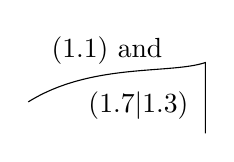
\begin{tikzpicture}[x=1cm,y=1cm]
\node at (0,.45) {$(1.1)$ and};
\node at (.4,-.25) {$(\unsure{1.7|1.3})$};
\draw (-1,-.2) .. controls (-.2,.3) and (.8,.15) .. (1.25,.3) -- (1.25,-.6);
\end{tikzpicture}}.

Let us return to $M^*$, and $L$ satisfying $(6.1)_i$. We have seen how \deleted{the} this condition implies the \uline{decomposition of} $M^*$ in \deleted{\unsure{canonical}} terms of primitive pieces
\[
\left\{\begin{aligned}
M^i&\simeq P^i+LP^{i-2}+L^2P^{i-4}\quad\text{---}\\
M^{2n-i}&\simeq L^{n-i}P^i+L^{n-i+1}P^{i-2}\quad\text{---}
\end{aligned}\right.\qquad\bigg|\quad\text{if }i\leq n
\tag{6.4}
\]
We denote by $\pi_{i,\alpha}$ the projection of $M^i$ onto $L^\alpha P^{i-2\alpha}$, by $\pi_{2n-i,\alpha}$ that of $M^{2n-i}$ onto $L^{n-i+\alpha}P^{i-2\alpha}$,
\mspage{8}
